\chapter{Theory}
In this section, the theoretical modelling of the bicycle and the data driven Min-Max MPC is discussed.

Since the objective of this research is to simply balance the bicycle, a simple kinetic model is sufficient for this purpose. We use two models and compare between them in terms of control and balance.
The difference between both models is considering the fork angle.
For controlling the bicycle, the data-driven MPC is compared with an LQR contoller and is applied in simulation and on a real model-scale bicycle to assess the controllers. In this chapter, the bicycle model used is discussed and the theory behind the data-driven state-feedback controller is explained.

\section{Bicycle Modelling}
\label{sec:bike_modelling}
	To model the riderless bicycle, it can be treated as an inverted pendulum. There are some (assumptions) parameters that are neglected such as: elasticity of bicycle parts, the tire-road friction, etc. A simple second-order model of the bicycle can be derived given that the rear-speed is constant, the bicycle rolling on the horizontal plane, and initially, the steer axis $\lambda$ is in a vertical position as in Figure \ref{fig:bike_model}. Using the Conservation of Angular Momentum, Equation \ref{eq:bike_second_order} is acquired to balance the bicycle. This is based on linearisation where the desired stability steady-state for both angles $\delta$ and $\phi$ is 0.
	\begin{equation}
		\label{eq:bike_second_order}
		\ddot{\varphi} - \frac{g}{h} \varphi = \frac{av \sin \lambda}{hl} \dot{\delta} + \frac{\left(v^2 h - ar_\tau g\right) \sin \lambda}{h^2 l} \delta
	\end{equation}
%	\varphi
	The state-space representation of the system given by Equation \ref{eq:bike_second_order} is given by
	\begin{equation}
		\label{eq:bike_state_equation}
		\begin{bmatrix}
			\dot{\varphi} \\
			\ddot{\varphi} \\
			\dot{\delta}
		\end{bmatrix}
		=
		\begin{bmatrix}
			0 & 1 & 0 \\
			\frac{g}{h} & 0 & \frac{\left(v^2 h - a r_\tau g\right) \sin \lambda}{h^2 l} \\
			0 & 0 & 0
		\end{bmatrix}
		\begin{bmatrix}
			\varphi \\
			\dot{\varphi} \\
			\delta
		\end{bmatrix}
		+
		\begin{bmatrix}
			0 \\
			\frac{a v \sin \lambda}{h l} \\
			1
		\end{bmatrix}
		\dot{\delta}.
	\end{equation}




	\change{Remove start}{}
	Bicycles:

	Models \cite{astrom2005bicycle}

	\textbf{Simple Second-Order Models}:

	\begin{itemize}
		\item Turn into codes later
		\item Self-Stabilization
		\item Manual Control
		\item Gyroscopic Effects
	\end{itemize}

	\textbf{Linear and Non-Linear Fourth order Models}

	Generate data using LQR feedback control:

	Using Bryson's rule to set Q and R:

	\begin{equation}
		Q = \begin{bmatrix}
			1 & 0 & 0 \\
			0 & 1 & 0 \\
			0 & 0 & 1
		\end{bmatrix},
		R = \begin{bmatrix}
			1
		\end{bmatrix}
	\end{equation}


	\change{Remove end}{}


\section{Data-Driven Min-Max MPC}
\label{sec:data_driven_mpc}

To formulate our problem, we consider a discrete-time linear time-invariant (LTI) system affected by process noise:
\[
x_{t+1} = A_s x_t + B_s u_t + \omega_t,
\]
where \(x_t \in \mathbb{R}^n\) is the state vector, \(u_t \in \mathbb{R}^m\) is the control input, and \(\omega_t \in \mathbb{R}^n\) represents unknown but bounded disturbance or noise at time \(t\).

The system matrices \(A_s\) and \(B_s\) are assumed to be unknown.
Instead of identifying a model explicitly, we utilize available noisy input-state data to design a stabilizing controller.
The noise \(\omega_t\) is assumed to satisfy:
\[
\|\omega_t\|_2^2 \leq \varepsilon,
\]
where \(\varepsilon \geq 0\) is a known bound.

\subsection{Set of Consistent System Matrices}

Given a sequence of collected input-state measurements, the set of all system matrices \((A, B)\) consistent with the data and noise bounds is characterized through a quadratic matrix inequality (QMI).
In particular, \((A, B)\) belongs to the set \(\mathcal{C}\) if and only if:
\[
\begin{bmatrix} I & A & B \end{bmatrix} \, \Pi(\tau) \, \begin{bmatrix} I & A & B \end{bmatrix}^\top \succeq 0,
\]
where \(\Pi(\tau)\) is a data-dependent matrix built from the available measurements and a set of non-negative scalars \(\tau\).

The construction of \(\Pi(\tau)\) ensures that all system matrices satisfying the observed data within the noise bounds are included.

\subsection{Min-Max Formulation}

The goal is to design a control law that stabilizes the system despite the uncertainty in \((A, B)\).
To achieve this, a min-max model predictive control (MPC) problem is formulated:
\unsure[inline]{Ask if min max is read RTL or LTR as in sup inf}{}
\[
\min_{u(\cdot)} \max_{(A, B) \in \mathcal{C}} \sum_{k=0}^{\infty} \ell(x_k, u_k),
\]
subject to the dynamics:
\[
x_{k+1} = A x_k + B u_k,
\]
where \(\ell(x, u) = x^\top Q x + u^\top R u\) is the quadratic stage cost, with weighting matrices \(Q \succ 0\) and \(R \succ 0\).

\subsection{State-Feedback Controller via Semidefinite Programming}

To reduce computational complexity and enable implementation on embedded platforms, a state-feedback control law of the form:
\[
u_t = K x_t
\]
is sought.

The optimal feedback gain \(K\) is obtained by solving a convex semidefinite program (SDP) derived from the min-max formulation.
Specifically, there exists a positive definite matrix \(P\) such that for all \((A, B) \in \mathcal{C}\), the following holds:
\[
(A + B K)^\top P (A + B K) - P + Q + K^\top R K \preceq 0.
\]
This inequality ensures that the closed-loop system is exponentially stable and satisfies the cost decrease condition.

The SDP formulation allows the computation of \(K\) directly from the noisy input-state data without requiring explicit model identification.

\todo[inline]{remove}
\subsection{Advantages of the Approach}

Compared to classical model-based MPC, the data-driven min-max MPC approach:
\begin{itemize}
	\item Provides robust stability guarantees even when the system model is unknown.
	\item Explicitly accounts for measurement noise in the controller design.
	\item Avoids over-conservatism typically found in robust tube-based MPC methods.
	\item Enables deployment on resource-limited hardware by using precomputed static feedback gains.
\end{itemize}

This method is particularly suitable for systems like the self-balancing mini-bicycle, where precise modeling is difficult due to parameter variations and unmodeled dynamics.
\begin{figure}
	\centering
	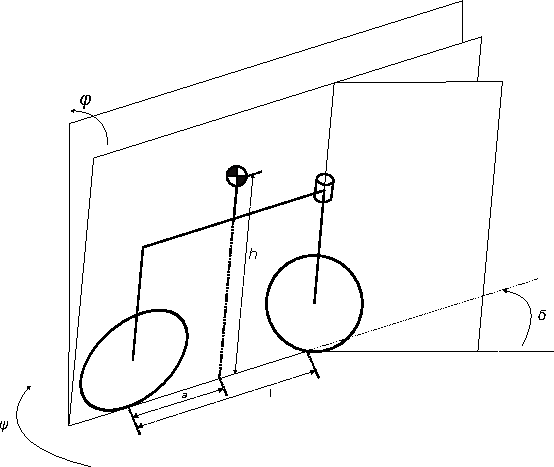
\includegraphics[width=0.7\linewidth]{figures/minibike/model.pdf}
	\caption{A Kinetic no-fork model of the bicycle}
	\label{fig:bike_model}
\end{figure}
\todo[inline]{Add the Fork Model simple drawing}
\begin{framed}
	\noindent
	\textbf{Main Optimization Problem: Data-Driven Min-Max MPC}

	\vspace{0.3em}
	Given collected input-state data and the corresponding consistent set of system matrices \(\mathcal{C}\),
	the data-driven min-max control problem seeks a state-feedback gain \(K\) minimizing the worst-case infinite-horizon cost:
	\[
	\min_{u(t)} \max_{(A, B) \in \mathcal{C}} \sum_{k=0}^{\infty} x_k^\top Q x_k + u_k^\top R u_k
	\]
	subject to the closed-loop dynamics:
	\[
	x_{k+1} = (A + B K) x_k
	\]
	and input-state constraints (if any).

	This is reformulated as a semidefinite program (SDP) that searches for a positive definite matrix \(P \succ 0\) and feedback gain \(K\) satisfying:
	\[
	(A + B K)^\top P (A + B K) - P + Q + K^\top R K \preceq 0, \quad \forall (A, B) \in \mathcal{C}.
	\]

	\vspace{0.5em}
	The resulting controller guarantees robust exponential stability and constraint satisfaction for all systems compatible with the observed data.
\end{framed}
